\appendix
\addcontentsline{toc}{chapter}{Appendices}
\startcontents
\startlist[appendix]{lof}
\startlist[appendix]{lot}
\printcontents{atoc}{0}{\chapter*{Appendices}}
\begingroup
\let\clearpage\relax
\singlespacing
\printlist[appendix]{lof}{}{\chapter*{List of Figures}}
\printlist[appendix]{lot}{}{\chapter*{List of Tables}}
\endgroup

\chapter{Appendices}
\label{app:Appendix}

\section{Additional tables}

\subsection{Chapter 5 Tables}

\begin{table}[htbp]
%\setlength{\tabcolsep}{20pt} only to stretch the columns if you want
%\renewcommand{\arraystretch}{1.5}
\centering
\begin{tabular}{@{} c c c c c}
\toprule
                   &                    &               & TSS enrichment &             \\
\textbf{Cell type} & \textbf{Condition} & \textbf{CTL1} & \textbf{CTL2} & \textbf{CTL3} \\
\midrule
\midrule
      & Fresh	 & 17.4 & 19.6 & 14.11\\
CD14	& Frozen & 26.3 & 25.2 & 27.1 \\
      & Fixed	 & 2.5  & 16.5 & 22.4 \\
\midrule
      & Fresh	 & 5.3  & 5.6  & 7.7 \\
CD4	  & Frozen & 17.9 & 14.1 & 16.1 \\
      & Fixed	 & 7.9  & 23.0 & 14.3 \\
\bottomrule
\end{tabular}
\medskip %gap
\caption[Enrichment of ATAC-seq reads across the TSS for the CD14$^+$ monocytes and CD4$^+$ samples fresh, frozen and fixed.]{\textbf{Enrichment of ATAC-seq reads across the TSS for the CD14$^+$ monocytes and CD4$^+$ samples fresh, frozen and fixed.}}
\label{tab:Core_ATAC_TSS_summary_table}
\end{table}
\bigskip %bigger space






\subsection{Chapter 4 Tables}

\begin{table}[htbp]
%\setlength{\tabcolsep}{20pt} only to stretch the columns if you want
%\renewcommand{\arraystretch}{1.5}
\centering
\begin{tabular}{@{} c c c}
\toprule
\textbf{Sample ID} & \textbf{NRF} & \textbf{PBC1/PBC2} \\
\midrule
\midrule
PS2000 CD14	& 77.6	& 0.60/2.5\\
PS2001 CD14	& 84.9	& 0.70/3.0\\
PS2314 CD14	& 81.1	& 0.60/1.8\\
PS2319 CD14	& 79.9	& 0.60/2.2\\
CTL7 CD14	  & 81.1	& 0.65/2.2\\
CTL8 CD14	  & 83.9	& 0.66/2.3\\
CTL9 CD14	  & 80.7	& 0.60/2.3\\
CTL10 CD14	& 83.1	& 0.65/2.1\\
\midrule
PS2000 CD4  & 84.8	& 0.75/3.4\\
PS2001 CD4	& 82.0	& 0.72/2.9\\
PS2314 CD4	& 82.9	& 0.71/2.8\\
PS2319 CD4	& 82.4	& 0.73/3.2\\
CTL7 CD4	  & 78.6	& 0.68/2.5\\
CTL8 CD4    & 81.8	& 0.71/2.9\\
CTL9 CD4    & 81.6	& 0.74/3.3\\
CTL10 CD4   & 77.6	& 0.61/1.9\\
\midrule
PS2000 CD8 & 77.0 &	0.76/4.5\\
PS2001 CD8 & 74.7 &	0.74/4.0\\
PS2314 CD8 & 74.2 &	0.75/4.1\\
PS2319 CD8 & 72.2 &	0.75/4.0\\
CTL7 CD8	 & 32.7 & 0.32/1.5\\
CTL8 CD8	 & 70.1 &	0.70/3.3\\
CTL9 CD8	 & 73.9 &	0.73/3.7\\
CTL10 CD8	 & 68.2 &	0.65/2.9\\
\midrule
PS2000 CD19	& 38.0 & 0.42/1.9\\
PS2001 CD19	& 71.4 & 0.71/3.7\\
PS2314 CD19	& 29.4 & 0.34/1.8\\
PS2319 CD19	& 76.1 & 0.78/4.8\\
CTL7	CD19  & 74.2	& 0.69/3.1\\
CTL8	CD19  & 68.4  &	0.67/3.2\\
CTL9	CD19  & 75.1  &	0.76/4.6\\
CTL10	CD19  & 61.7  & 0.59/2.6\\
\bottomrule
\end{tabular}
\medskip %gap
\caption[Evaluation of ChiPm library complexity for the psoriasis and control chort 1B ChIPm assay.]{\textbf{Evaluation of ChiPm library complexity for the psoriasis and control chort 1B ChIPm assay.} NRF, PBC1 and PBC2 are the three measures used according to the ENCODE standards as referred in Chapter \ref{ch:Mat}. 0.5$\leq$NRF$<$0.8 acceptable; 0.8$\leq$NRF$\leq$0.9 compliant; NRF$>$0.9 ideal; 0.5$\leq$PBC1$<$0.8 and 1$\leq$PBC2$<$3 moderate bottlenecking; 0.8$\leq$PBC1$<$0.9 and 3$\leq$PBC2$<$10 mild bottlenecking.}
\label{tab:ChIPm_PS_CTL_library_complexity}
\end{table}
\bigskip %bigger space

\begin{table}[htbp]
%\setlength{\tabcolsep}{20pt} only to stretch the columns if you want
%\renewcommand{\arraystretch}{1.5}
\centering
\begin{tabular}{@{} c }
\toprule
\textbf{CD14$^+$ monocytes additional enriched pathways in psoriasis} \\
\midrule
\midrule
Generic transcription \\
RNA transport \\
GnRH signalling \\
Ribosome biogenesis in eukaryotes \\
Neurotrophin signaling \\
Spliceosome \\
Autophagy \\
Protein processing in endoplasmic reticulum \\
                        \\
\textbf{CD8$+$ additional enriched pathways in psoriasis} \\
\midrule
\midrule
Epstein-Barr virus infection \\
RNA Polymerase I and III, and mitochondrial transcription\\
Apoptosis \\
\bottomrule
\end{tabular}
\medskip %gap
\caption[Additional enriched pathways for DEGs between psoriasis and healthy controls in CD14$^+$ monocytes and CD8$^+$ cells.]{\textbf{Additional enriched pathways DEGs between psoriasis and healthy controls in CD14$^+$ monocytes and CD8$^+$ cells.} Significant pathways for FDR$<$0.01. All the enriched pathways contained a minimum of ten DEGs FDR$<$0.05 from the analysis.}
\label{tab:RNAseq_PS_CTL_additional_pathways}
\end{table}



\begin{table}[htbp]
%\setlength{\tabcolsep}{20pt} only to stretch the columns if you want
%\renewcommand{\arraystretch}{1.5}
\centering
\begin{tabular}{@{} c }
\toprule
\textbf{Lesional versus uninvolved epidermis additional enriched pathways} \\
\midrule
\midrule
Genes encoding extracellular matrix and extracellular matrix-associated proteins \\ 
Serine/threonine-protein kinase (PLK1) signalling \\
Genes encoding secreted soluble factors \\
Glycolysis/gluconeogenesis \\
FOXM1 transcription factor network \\
Phase 1 functionalization of compounds \\
Biological oxidations \\
G2/M Checkpoints \\
Biological oxidations \\
Aurora B signaling \\
Chemical carcinogenesis \\
Serotonergic synapse \\
Drug metabolism-cytochrome P450 \\
Mitotic M-M/G1 phases \\
DNA Replication \\
MicroRNAs in cancer \\
Metabolism of amino acids and derivatives \\
Metabolism of carbohydrates \\
Glycosaminoglycan metabolism \\
E2F transcription factor network \\
p73 transcription factor network \\
Genes encoding structural ECM glycoproteins \\
Transmembrane transport of small molecules \\
Fc-epsilon receptor I signaling in mast cells \\
Tight junction \\
Origin recognition complex subunit 1 (Orc1) removal from chromatin \\
\bottomrule
\end{tabular}
\medskip %gap
\caption[Additional enriched pathways for DEGs between lesional and uninvolved epidermis isolated from psoriasis patients skin biopsies.]{\textbf{Additional enriched pathways for DEGs between lesional and uninvolved epidermis isolated from psoriasis patients skin biopsies.} Significant pathways for FDR$<$0.005. All the enriched pathways contained a minimum of ten DEGs FDR$>$0.05 from the analysis.}
\label{tab:RNAseq_PS_lesional_uninvolved_additional_pathways}
\end{table}




\subsection{Chapter 5 Tables}

\begin{table}[htbp]
%\setlength{\tabcolsep}{20pt} only to stretch the columns if you want
%\renewcommand{\arraystretch}{1.5}
\centering
\begin{tabular}{@{} c }
\toprule
\textbf{CC-mixed CD14$+$ monocytes additional enriched pathways} \\
\midrule
\midrule
SLE \\
Translation \\
3'-UTR-mediated translational regulation \\
Th-1 and Th-2 cell differentiation \\
Peptide chain elongation \\
Rheumatoid arthritis \\
Metabolism of proteins \\
Cell adhesion molecules (CAMs) \\
Th-17 cell differentiation \\
Nonsense mediated decay enhanced by the exon junction complex \\
SRP-dependent co-translational protein targeting to membrane \\
Hemostasis \\
Metabolism of mRNA \\
Platelet activation, signalling and aggregation \\
HTLV-I infection \\
Innate immune system \\
Adaptive immune system \\
                        \\
\textbf{CC-IL7R CD14$+$ monocytes additional enriched pathways} \\
\midrule
\midrule
SLE \\
Tuberculosis \\
Epstein-Barr virus infection \\
Immune System \\
\bottomrule
\end{tabular}
\medskip %gap
\caption[Additional enriched pathways for the DEGs between SF and PB CD14$^+$ monocytes from the CC-mixed and CC-IL7R subpopulations.]{\textbf{Additional enriched pathways for the DEGs between SF and PB CD14$^+$ monocytes from the CC-mixed and CC-IL7R subpopulations.} All the enriched pathways contained a minimum of ten DEGs from the analysis and were significant at an FDR$<$0.01.}
\label{tab:PSA_scRNAseq_CC_mixed_and_IL7R_additional_pathways}
\end{table}




\section{Additional figures}

\subsection{Chapter 3 Figures}
\begin{figure}[htbp]
\centering
\begin{subfigure}{0.70\textwidth}
\centering
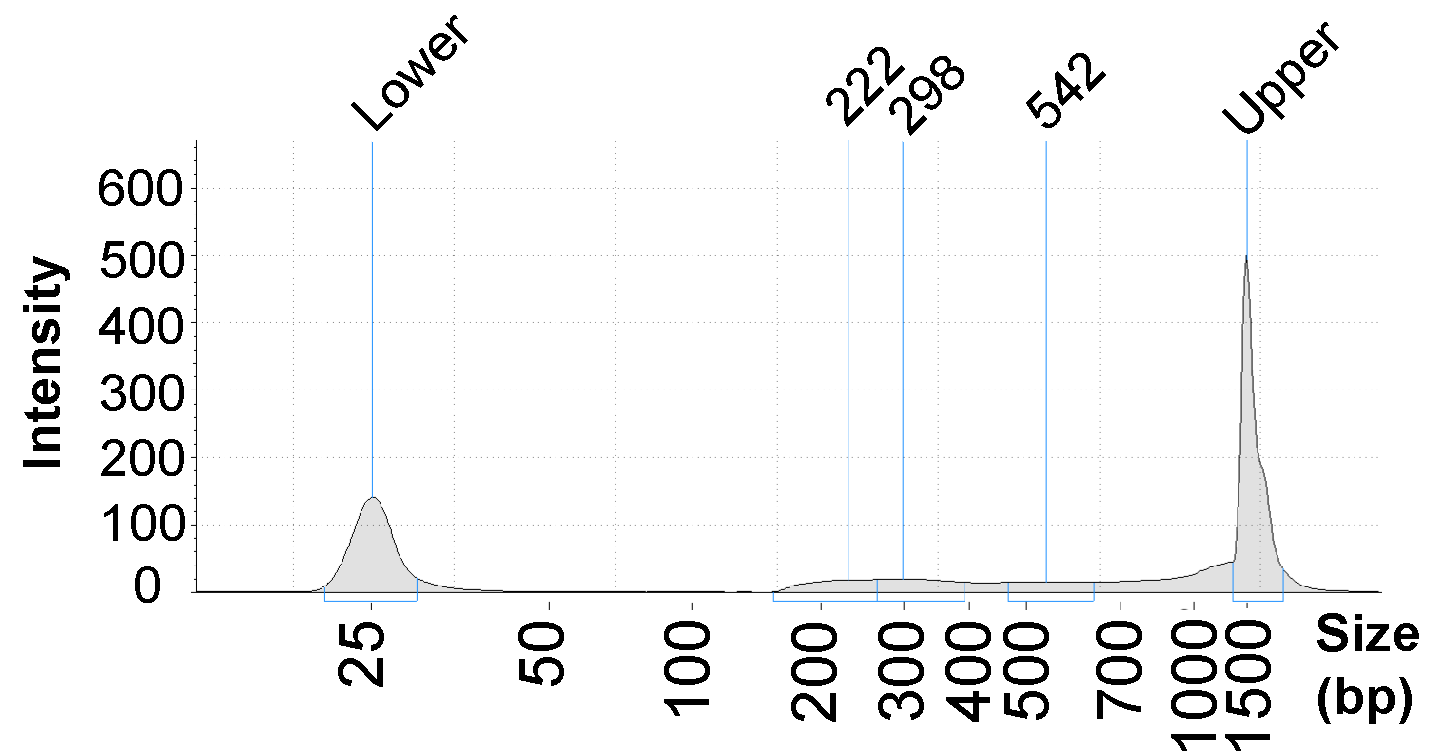
\includegraphics[width=\textwidth]{./Appendix/pdfs/Chapter3/FAST_ATAC_skin_tapestation_C1}
\caption{\textbf{}}
% The percentage sign indicated that the other subfig goes side by side
\end{subfigure}
\begin{subfigure}{0.70\textwidth}
\centering
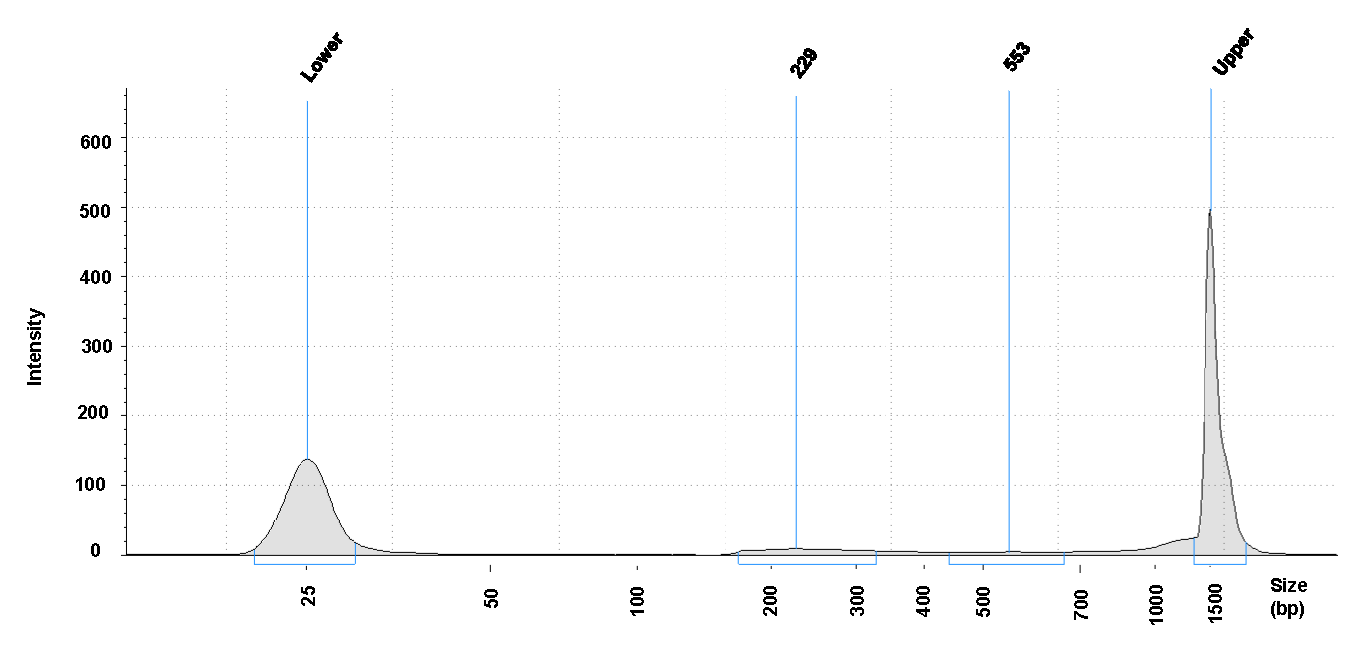
\includegraphics[width=\textwidth]{./Appendix/pdfs/Chapter3/FAST_ATAC_skin_tapestation_C3}
\caption{\textbf{}}
\end{subfigure}
\begin{subfigure}{0.70\textwidth}
\centering
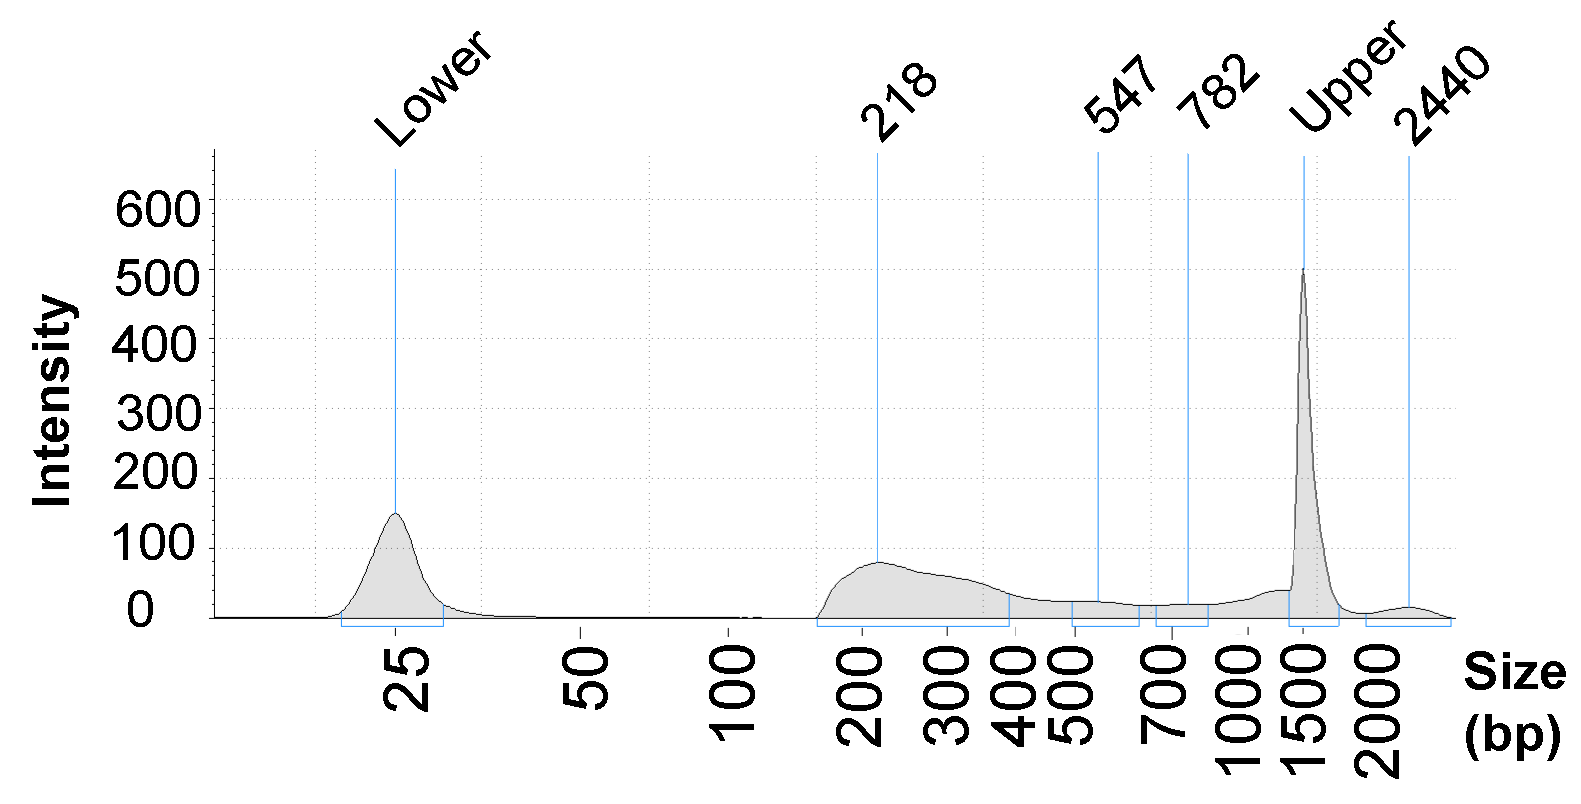
\includegraphics[width=\textwidth]{./Appendix/pdfs/Chapter3/FAST_ATAC_skin_tapestation_C4}
\caption{\textbf{}} % to add text to the figure name
\end{subfigure}
\begin{subfigure}{0.70\textwidth}
\centering
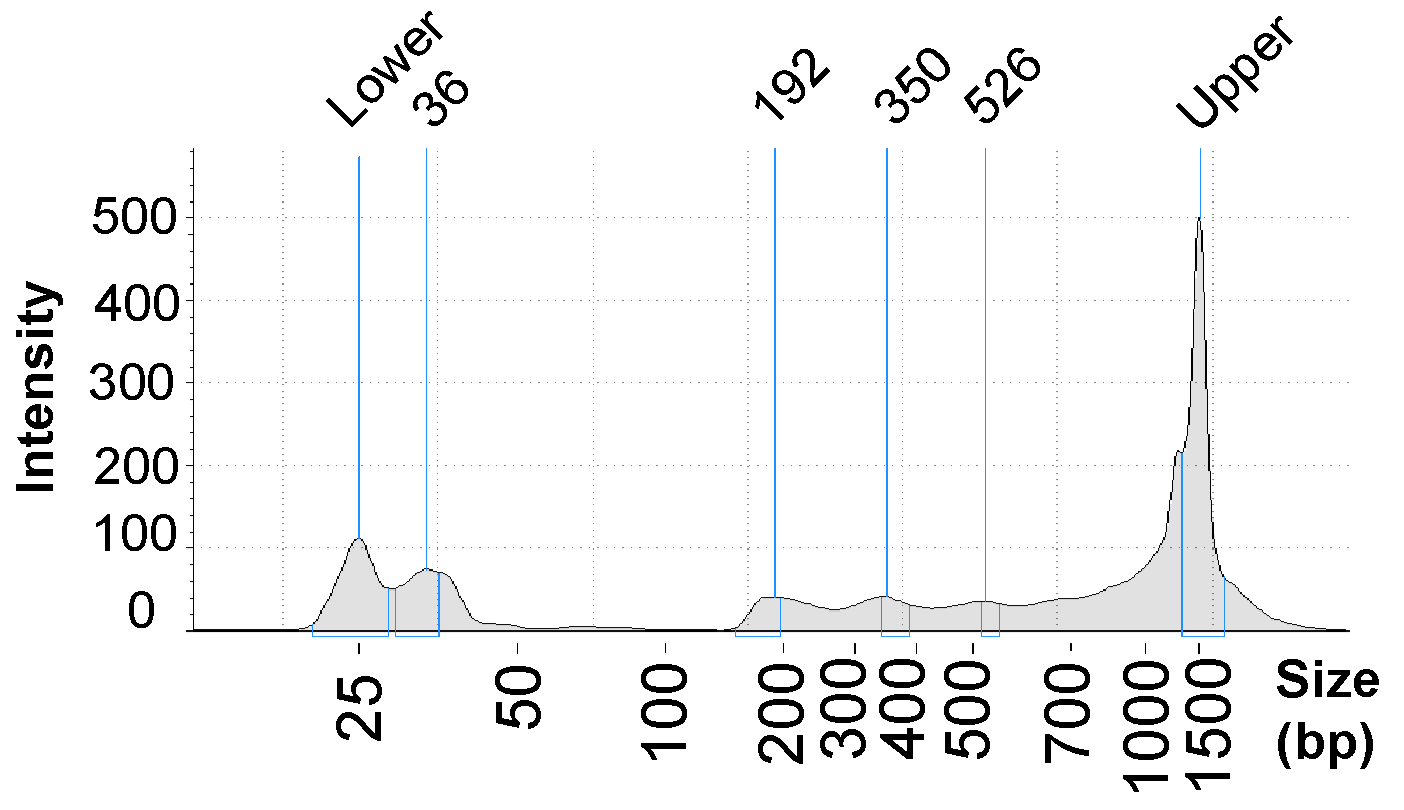
\includegraphics[width=\textwidth]{./Appendix/pdfs/Chapter3/Omni_ATAC_NHEK_Rep1_tapestation}
\caption{\textbf{}} % to add text to the figure name
\end{subfigure}
\hfill
\caption[FAST-ATAC and Omni-ATAC NHEK tapestation profiles.]{\textbf{FAST-ATAC and Omni-ATAC NHEK tapestation profiles.} \\
}
\label{fig:NHEK_tapestation}
\end{figure}



\begin{figure}[htbp]
\centering
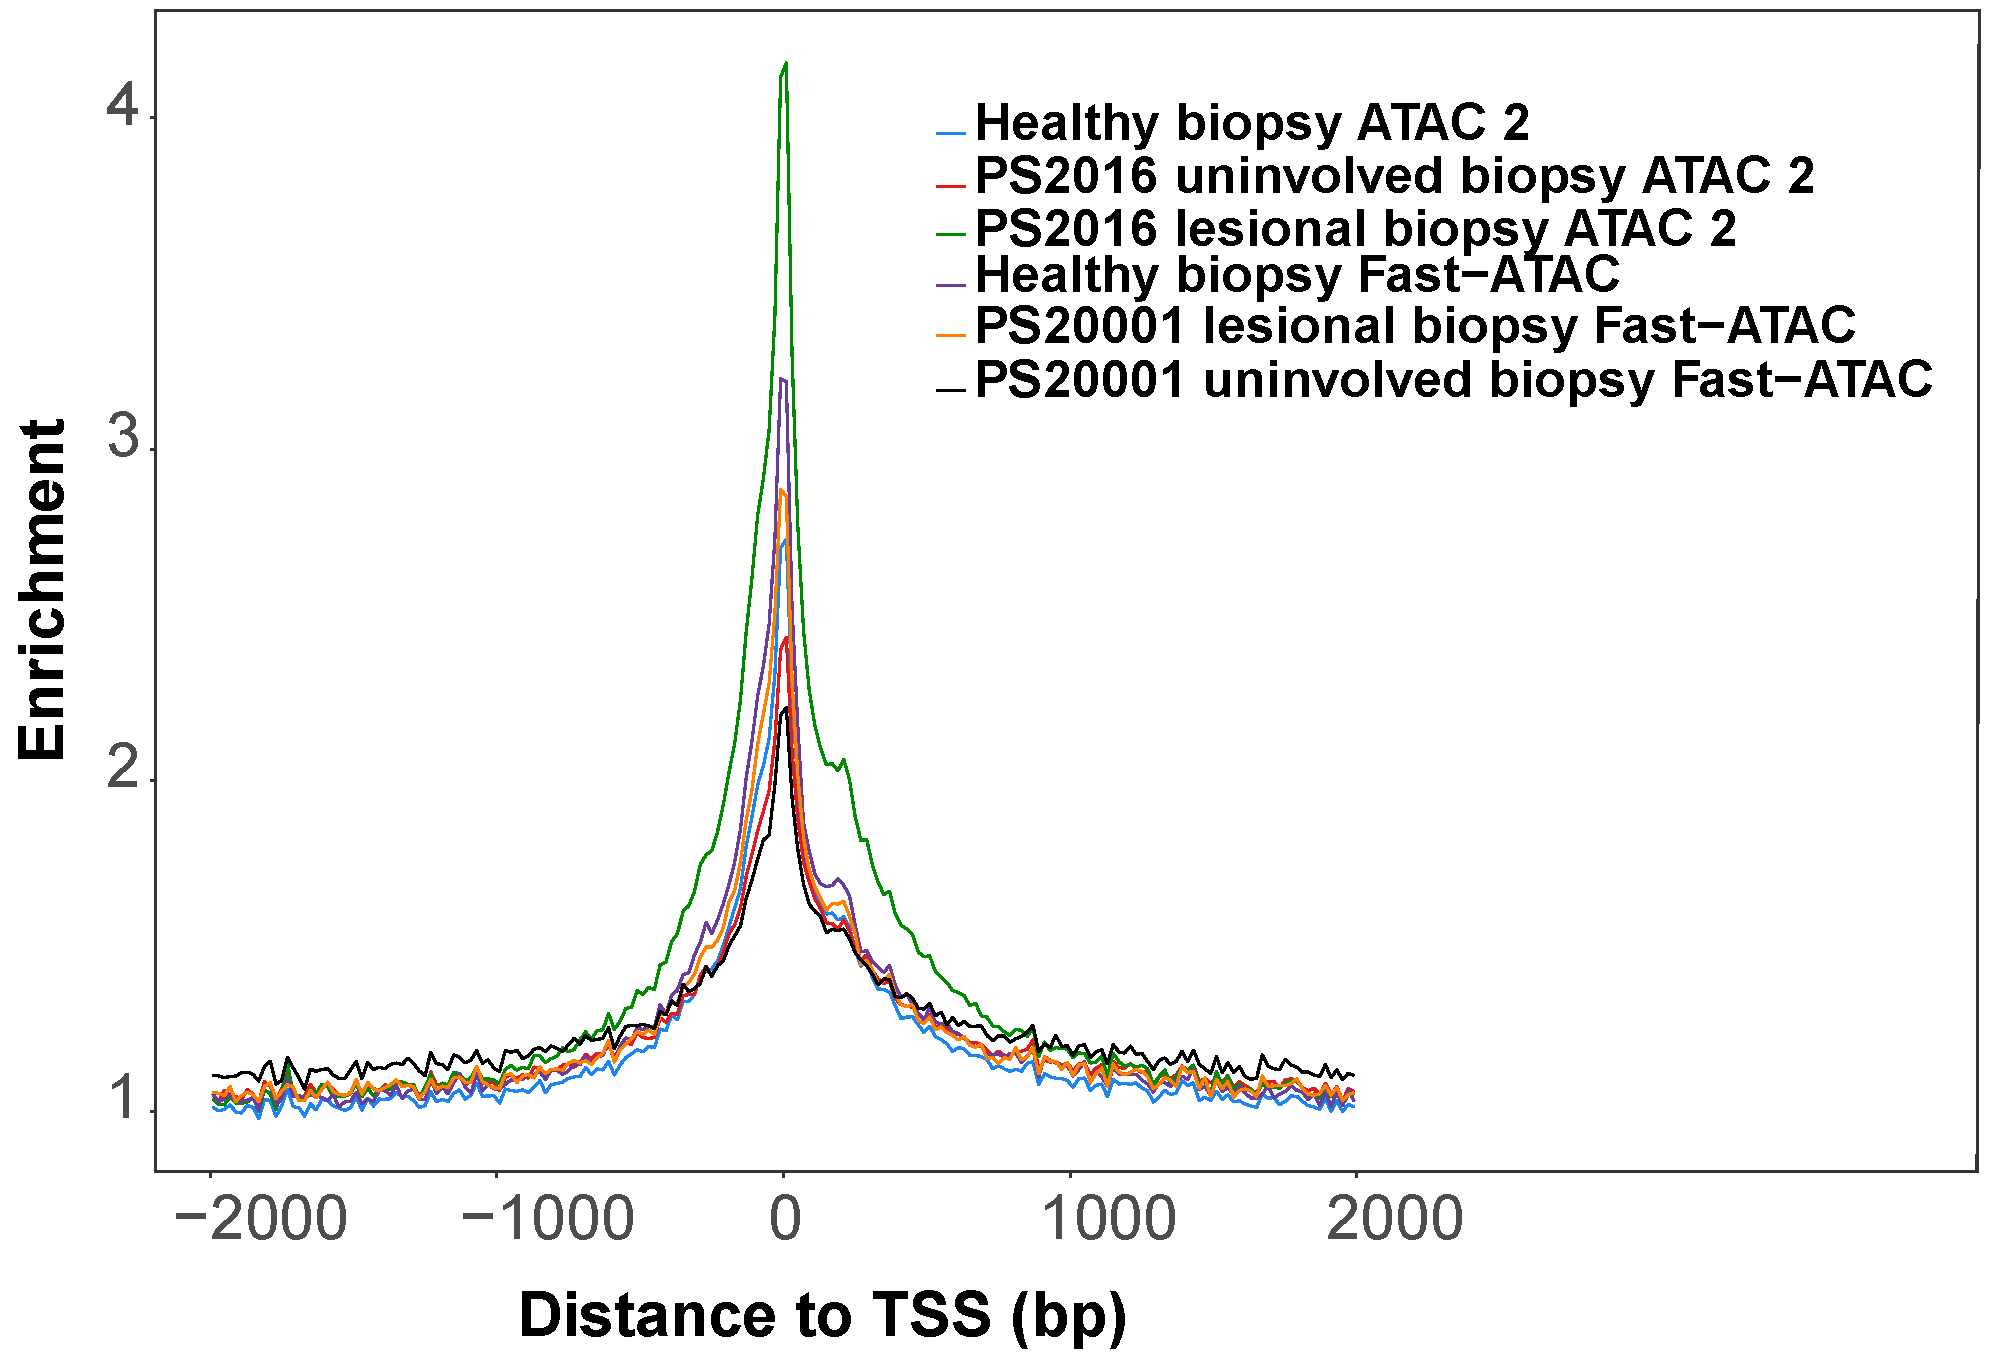
\includegraphics[width=0.8\textwidth]{./Appendix/pdfs/Chapter3/ATAC_skin_biopsy_samples_all_methods_TSS_enrichment_supplementary}
\caption[Assessment of TSS enrichment from ATAC-seq and FAST-ATAC in healthy and psoriasis skin biopsies samples.]{\textbf{Assessment of TSS enrichment from ATAC-seq and FAST-ATAC in healthy and psoriasis skin biopsy samples.}  }
\label{fig:TSS_skin_biopsies}
\end{figure}


\subsection{Chapter 4 Figures}

\begin{figure}[htbp]
\centering
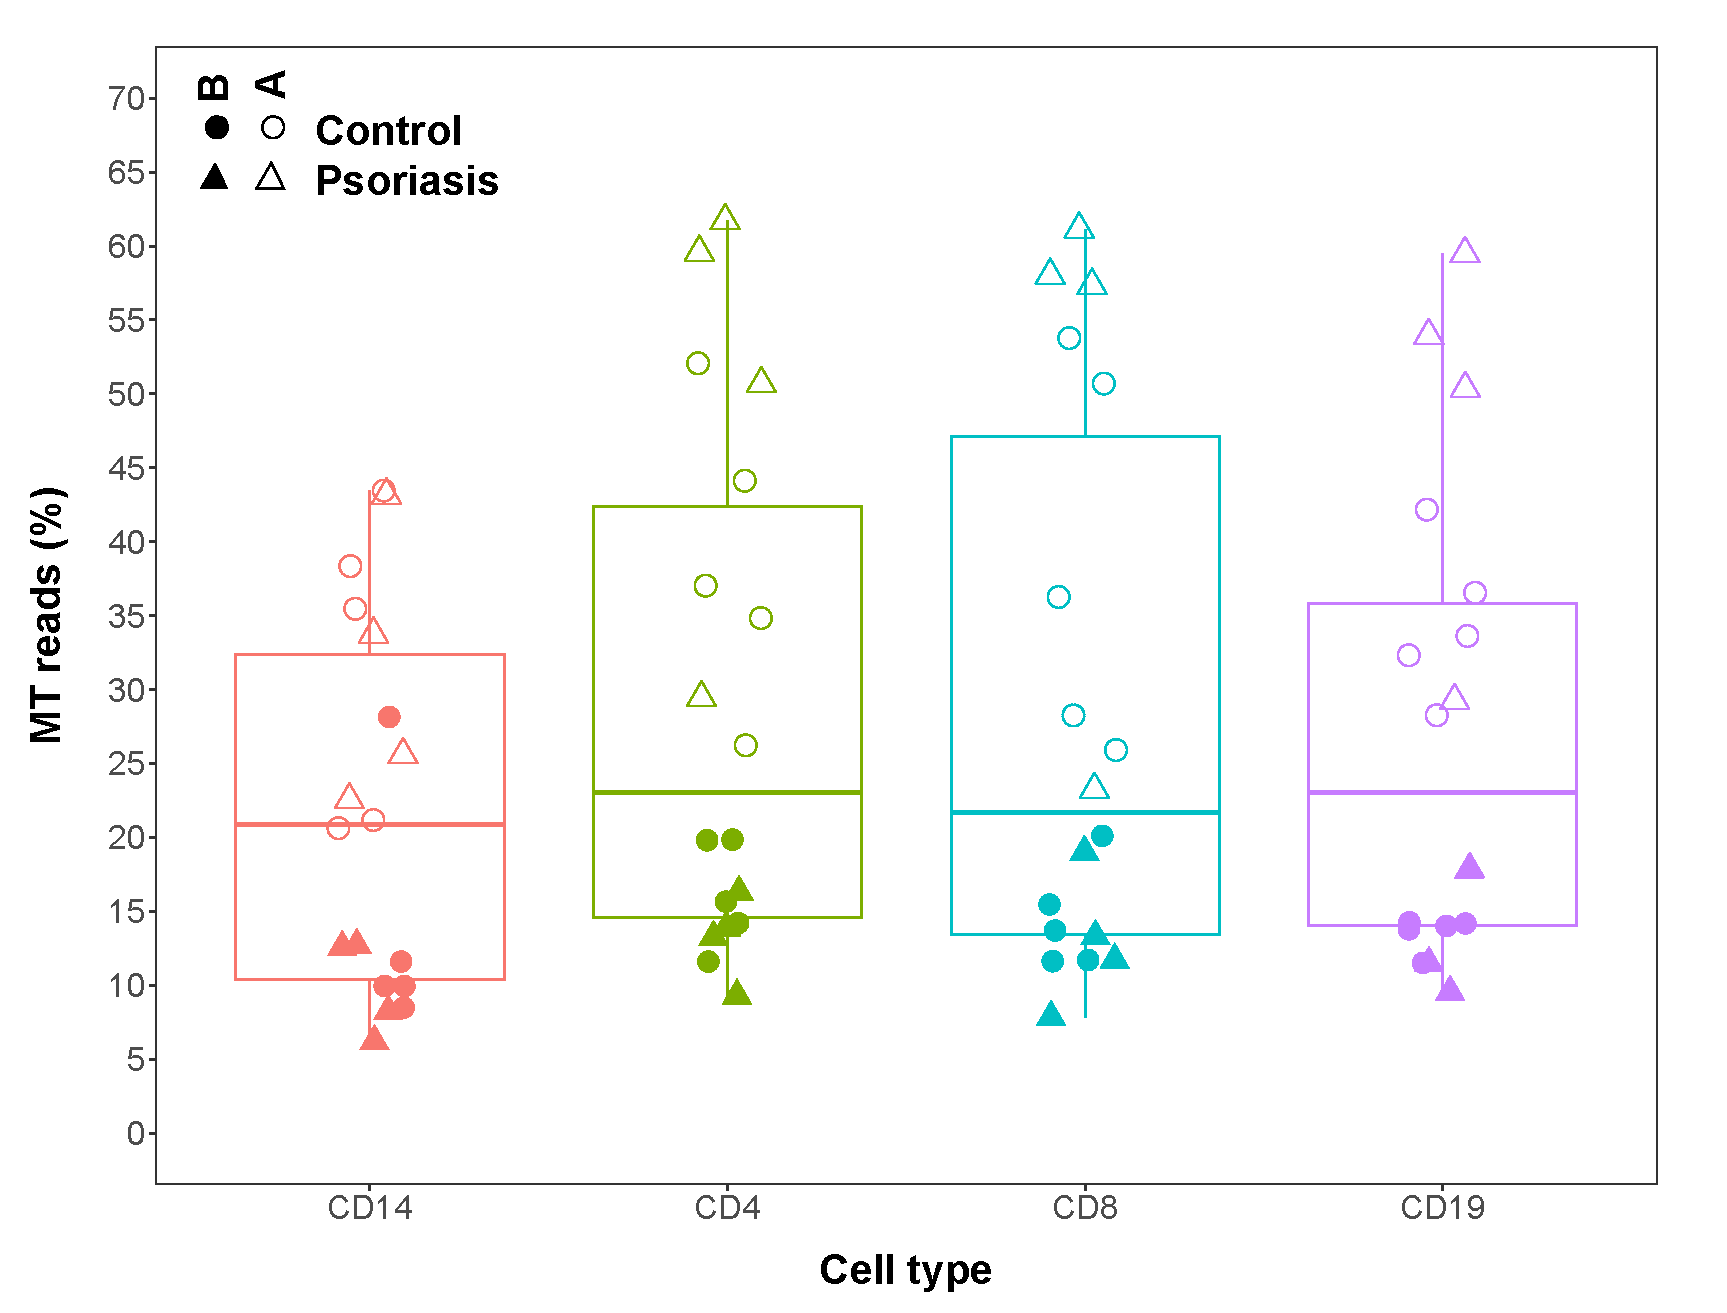
\includegraphics[width=0.6\textwidth]{./Appendix/pdfs/Chapter4/ATAC_PS_CTL_MT_percent_boxplot}
\caption[Percentage of MT reads in the ATAC-seq libraries generated in CD14$^+$ monocytes, CD4$^+$, CD8$^+$ and CD19$^+$ isolated from psoriasis patients and healthy controls.]{\textbf{Percentage of MT reads in the ATAC-seq samples generated in CD14$^+$ monocytes, CD4$^+$, CD8$^+$ and CD19$^+$ isolated from psoriasis patients and healthy controls.} Samples from cohort 1A (open circlues and triangles) were generated with the standard ATAC-seq protocol from Buenrostro \textit{et al.}, 2013 whereas samples from cohort 1B (filles circles and triangles) were processed using FAST-ATAC \parencite{Corces2016}.}
\label{fig:ATAC_PS_CTL_MT_percent}
\end{figure}


\begin{figure}[htbp]
\centering
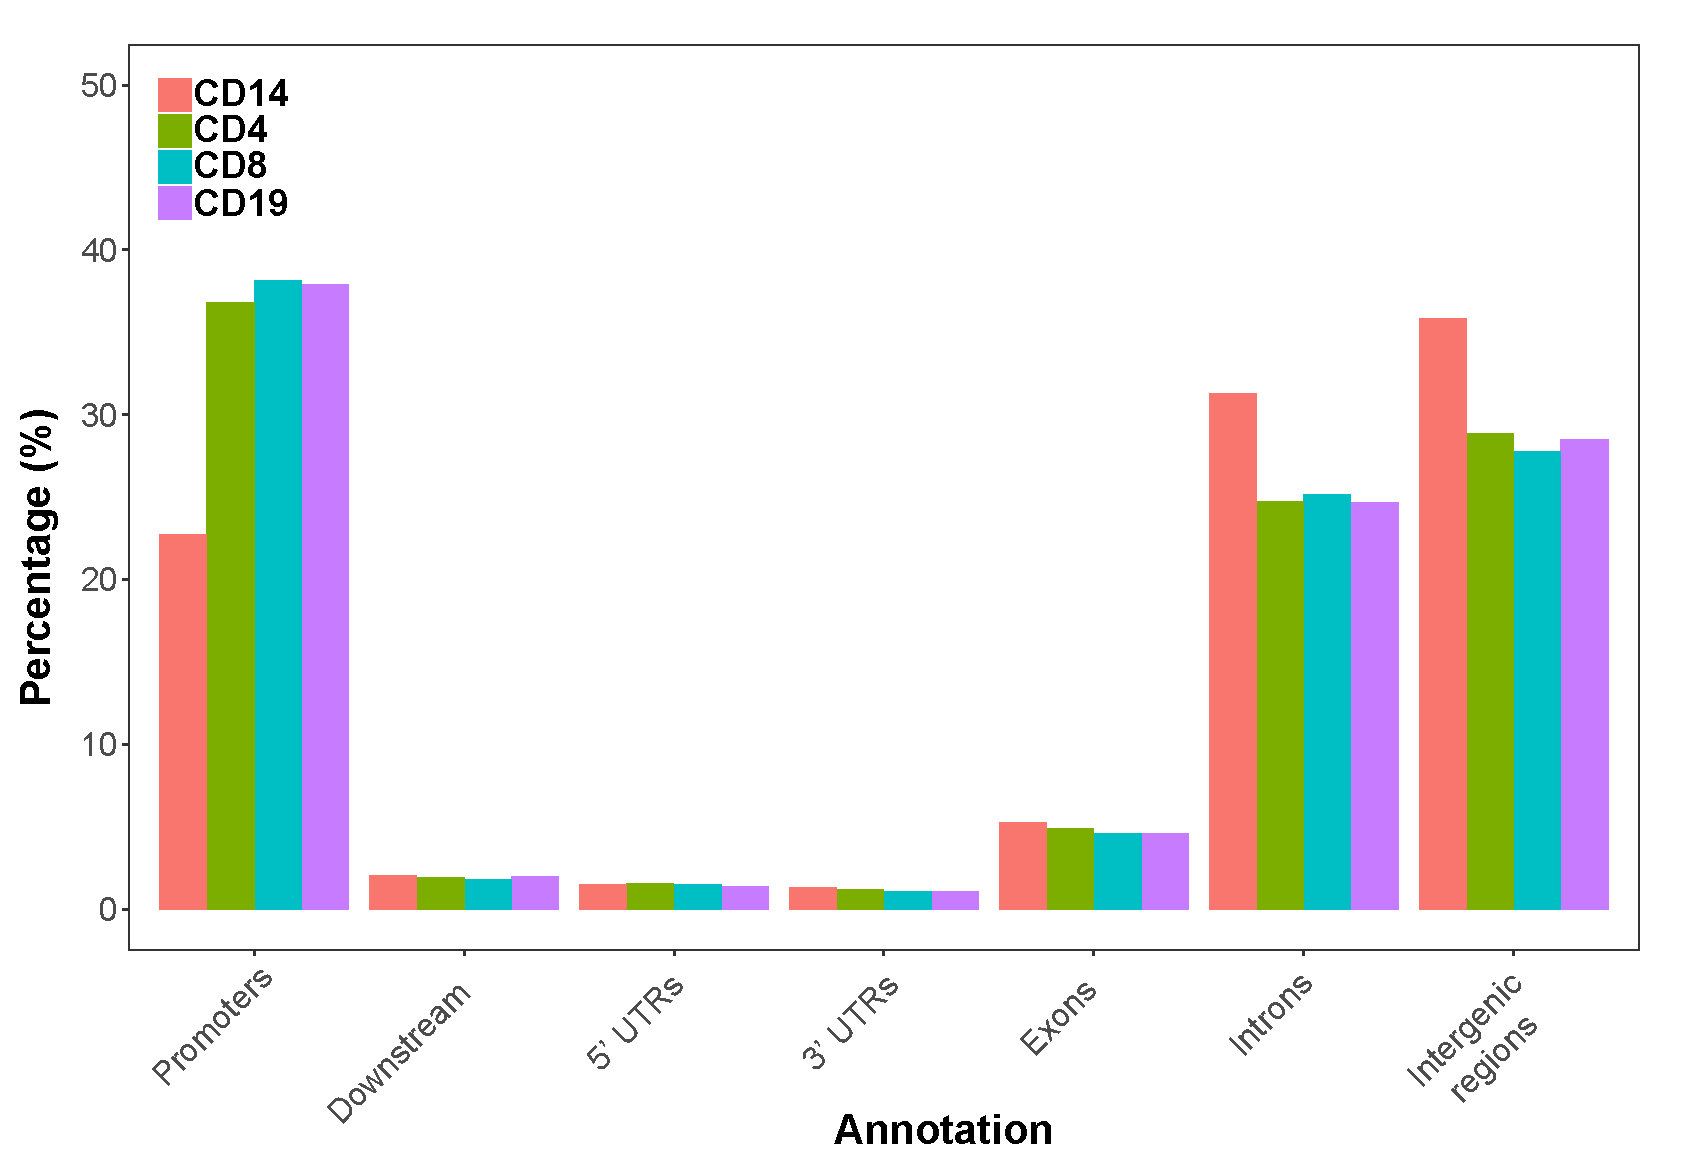
\includegraphics[width=0.6\textwidth]{./Appendix/pdfs/Chapter4/ATAC_all_cell_types_individual_master_lists_general_peak_annotation}
\caption[Genomic annotation of the consensus master list of ATAC-seq enriched sites built for downstream differential chromatin accessibility analysis in CD14$^+$ monocytes, CD4$^+$, CD8$^+$ and CD19$^+$.]{\textbf{Genomic annotation of the consensus master list of ATAC-seq enriched sites built for downstream differential chromatin accessibility analysis in CD14$^+$ monocytes, CD4$^+$, CD8$^+$ and CD19$^+$.} Annotation is expressed in percentage over the total number of ATAC-seq sites included in each particular cell type master list.}
\label{fig:ATAC_PS_CTL_genomic_annotation}
\end{figure}


\bigskip
\begin{figure}[H]
\centering
\begin{subfigure}[b]{0.70\textwidth}
\centering 
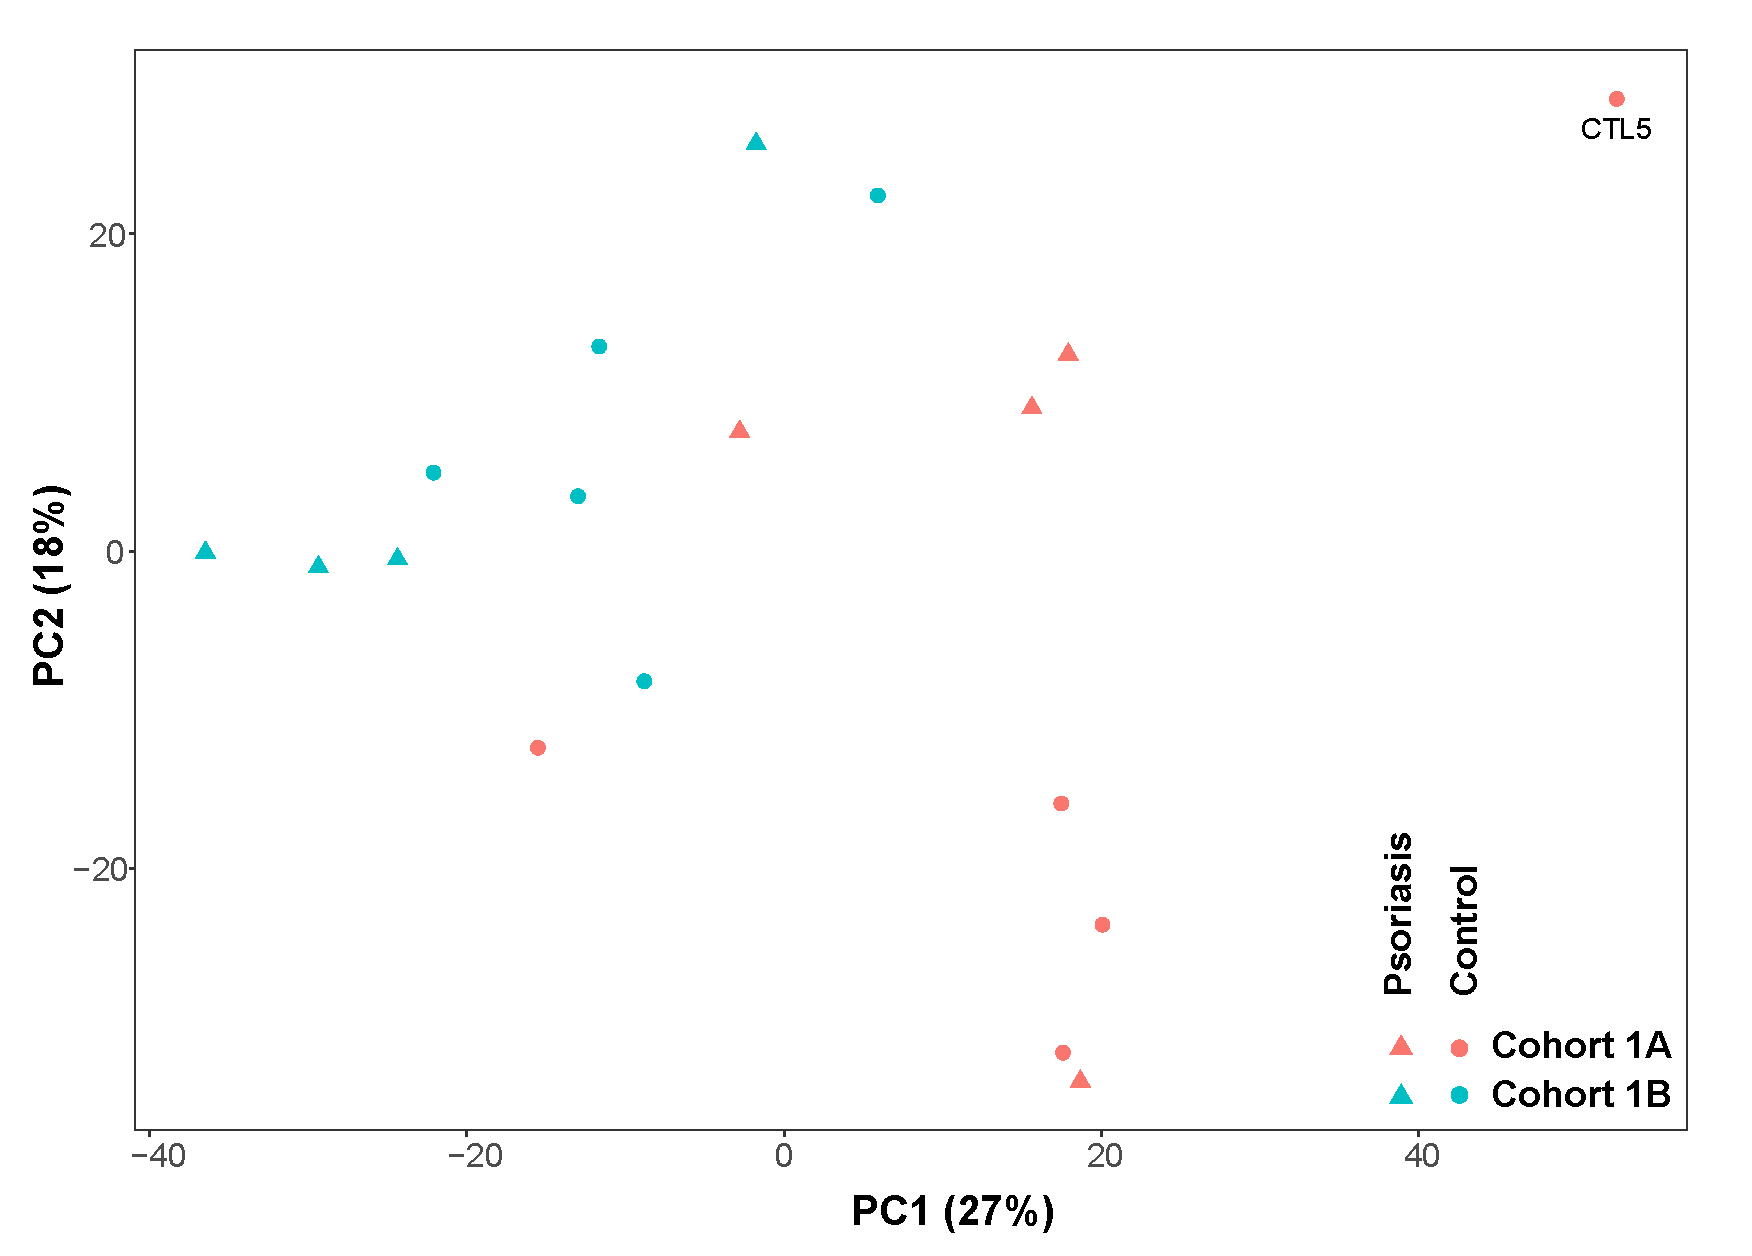
\includegraphics[width=\textwidth]{./Appendix/pdfs/Chapter4/ATAC_CD8_PS_CTL_PCA}
\caption{}
\end{subfigure}
~
\begin{subfigure}[b]{0.70\textwidth} 
%the [b] prevents offset in subcaptions
\centering
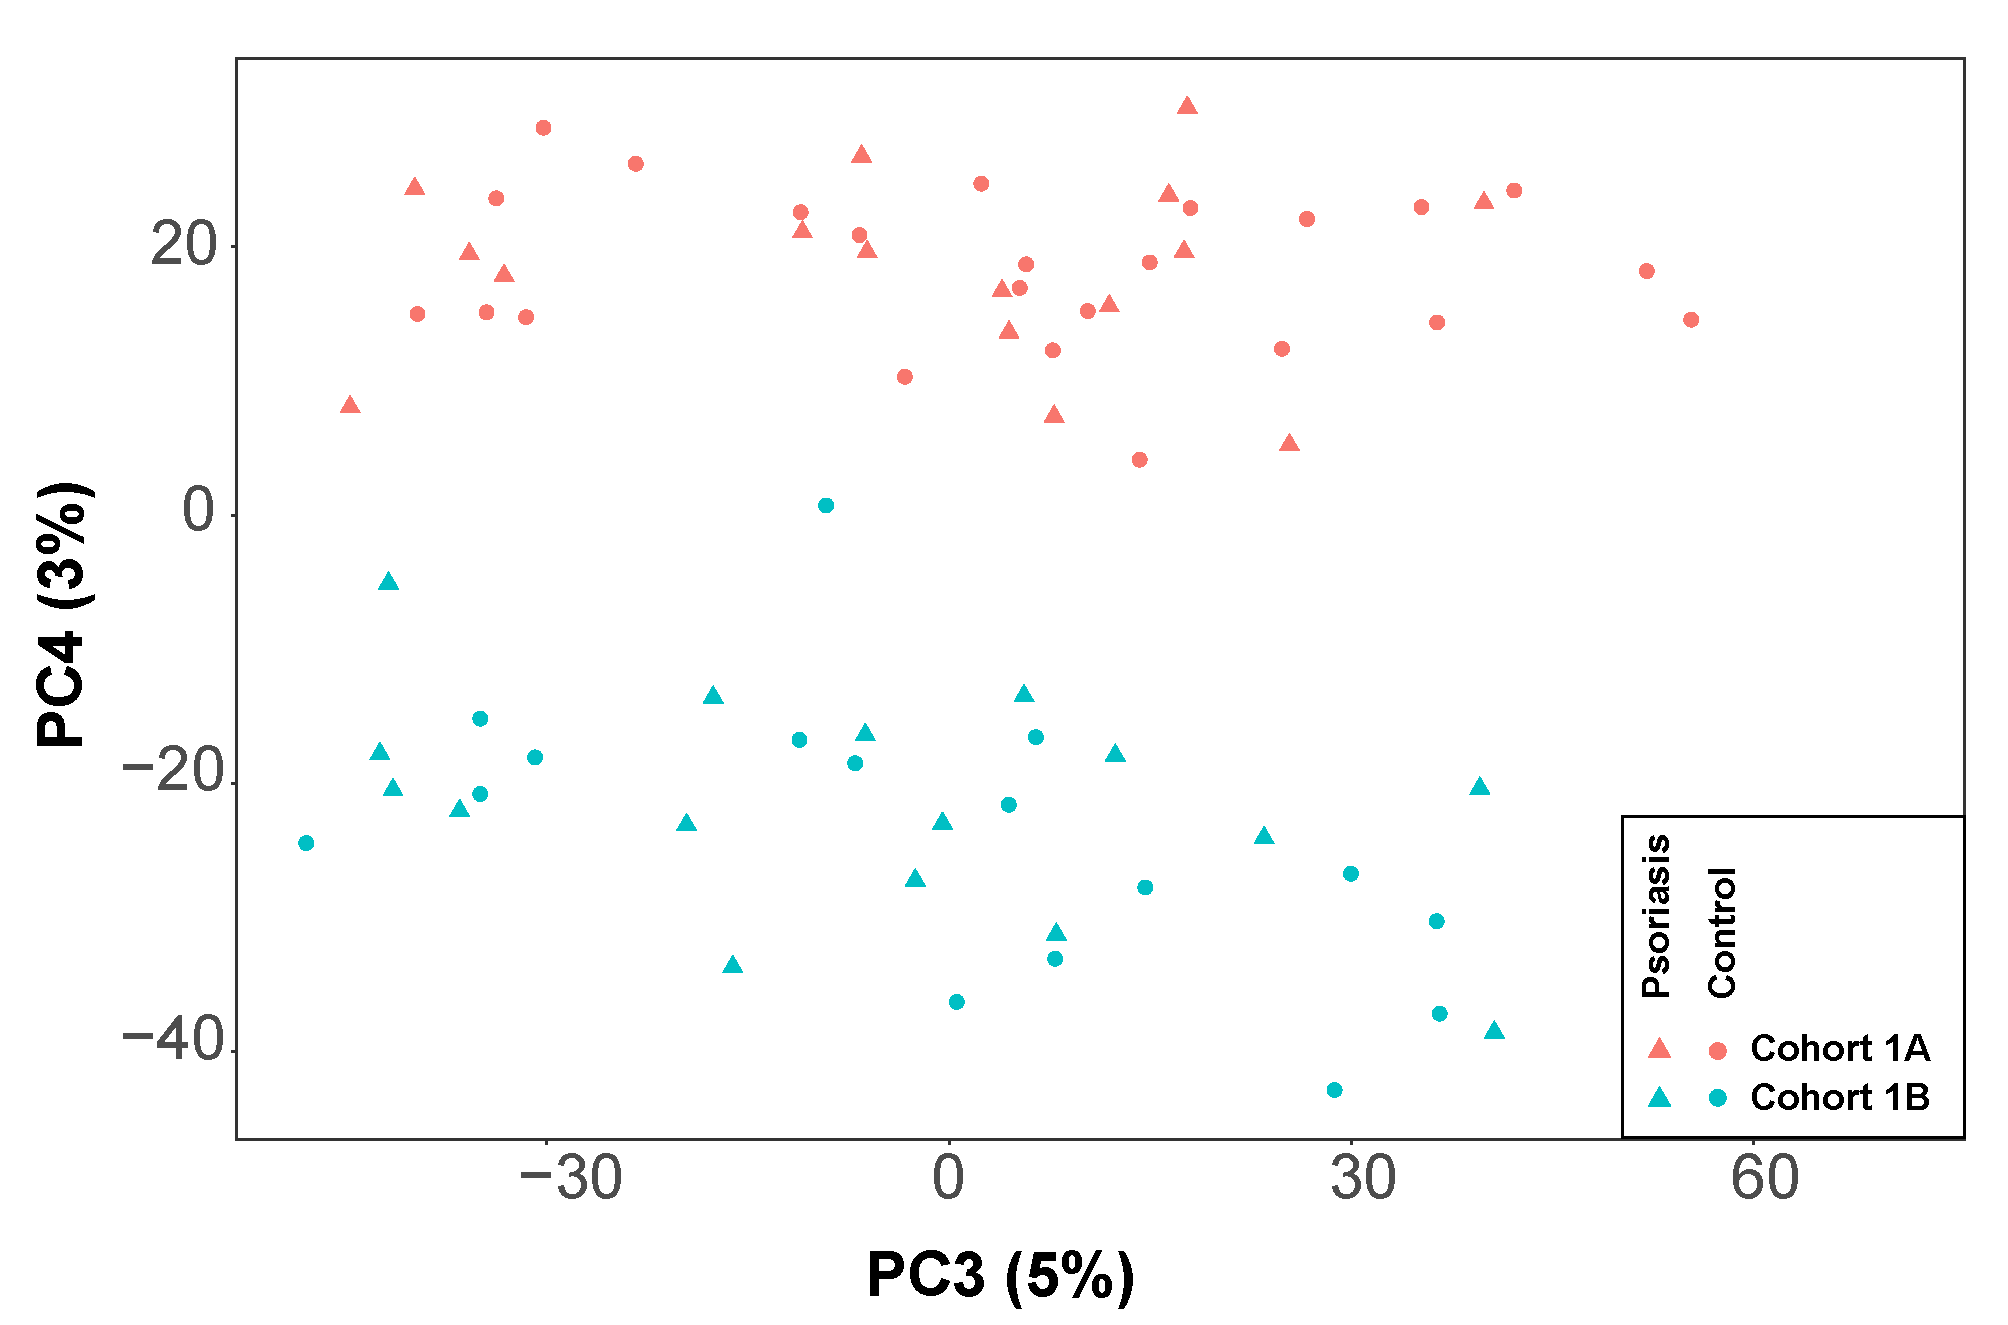
\includegraphics[width=\textwidth]{./Appendix/pdfs/Chapter4/PS_CTL_all_samples_varied_PCA3and4_plot}
\caption{}
\end{subfigure}
\caption[PCA analysis illustrating batch effect in ATAC-seq and RNA-seq samples.]{\textbf{PCA analysis illustrating batch effect in ATAC-seq and RNA-seq samples.} a) xxxx  b)}
\label{figure:ATAC_RNAseq_batch_effect}
\end{figure}



\subsection{Chapter 5 Figures}

\bigskip
\begin{figure}[H]
\centering
\begin{subfigure}[b]{0.45\textwidth}
\centering 
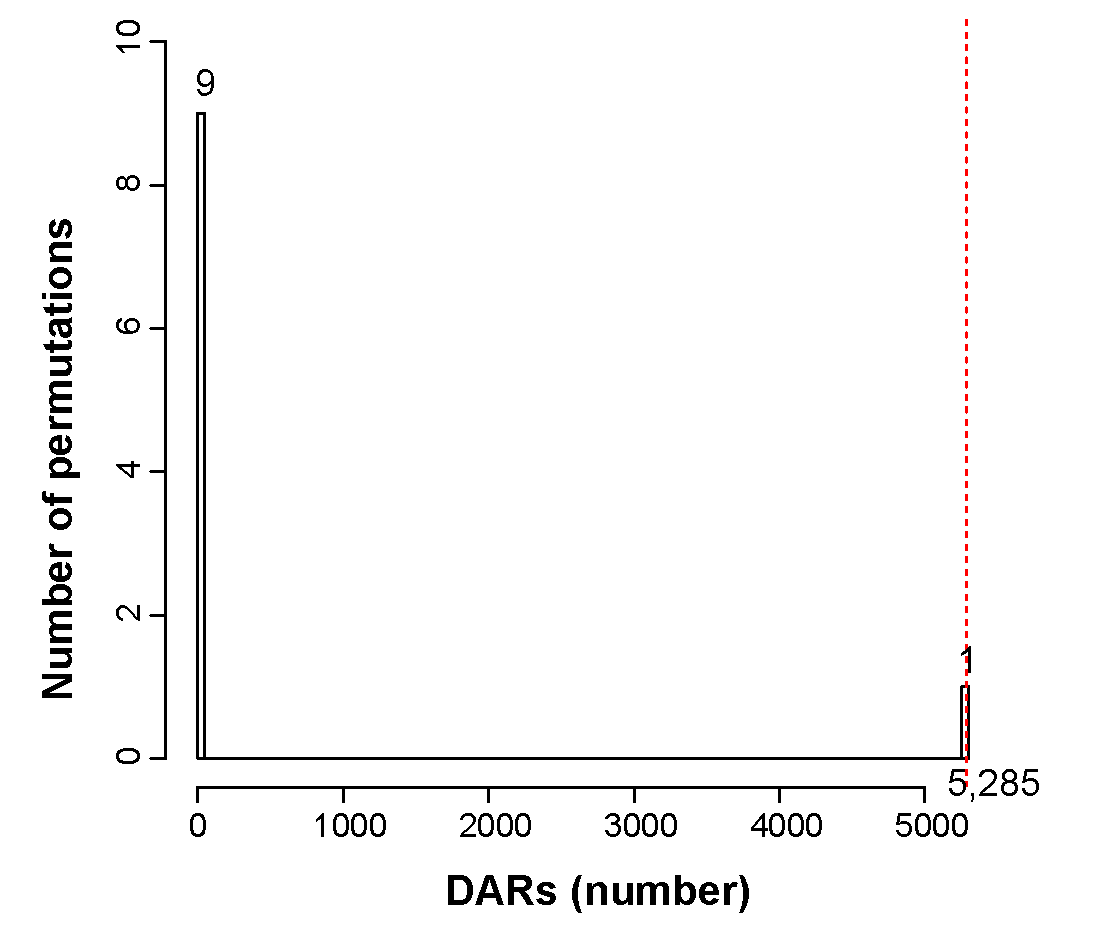
\includegraphics[width=\textwidth]{./Appendix/pdfs/Chapter5/ATAC_PsA_CD14_permutation_analysis}
\caption{}
\end{subfigure}
~
\begin{subfigure}[b]{0.45\textwidth}
\centering 
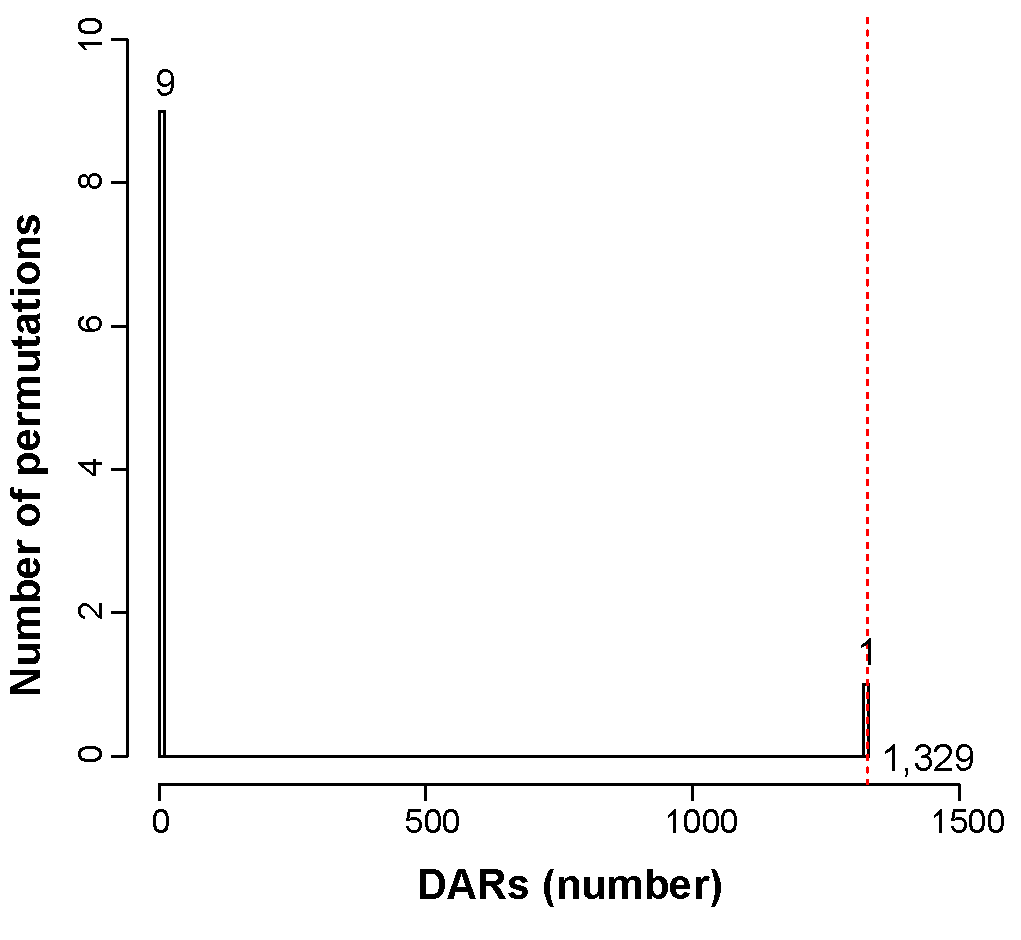
\includegraphics[width=\textwidth]{./Appendix/pdfs/Chapter5/ATAC_PsA_CD4_permutation_analysis}
\caption{}
\end{subfigure}
~
\begin{subfigure}[b]{0.45\textwidth} 
%the [b] prevents offset in subcaptions
\centering
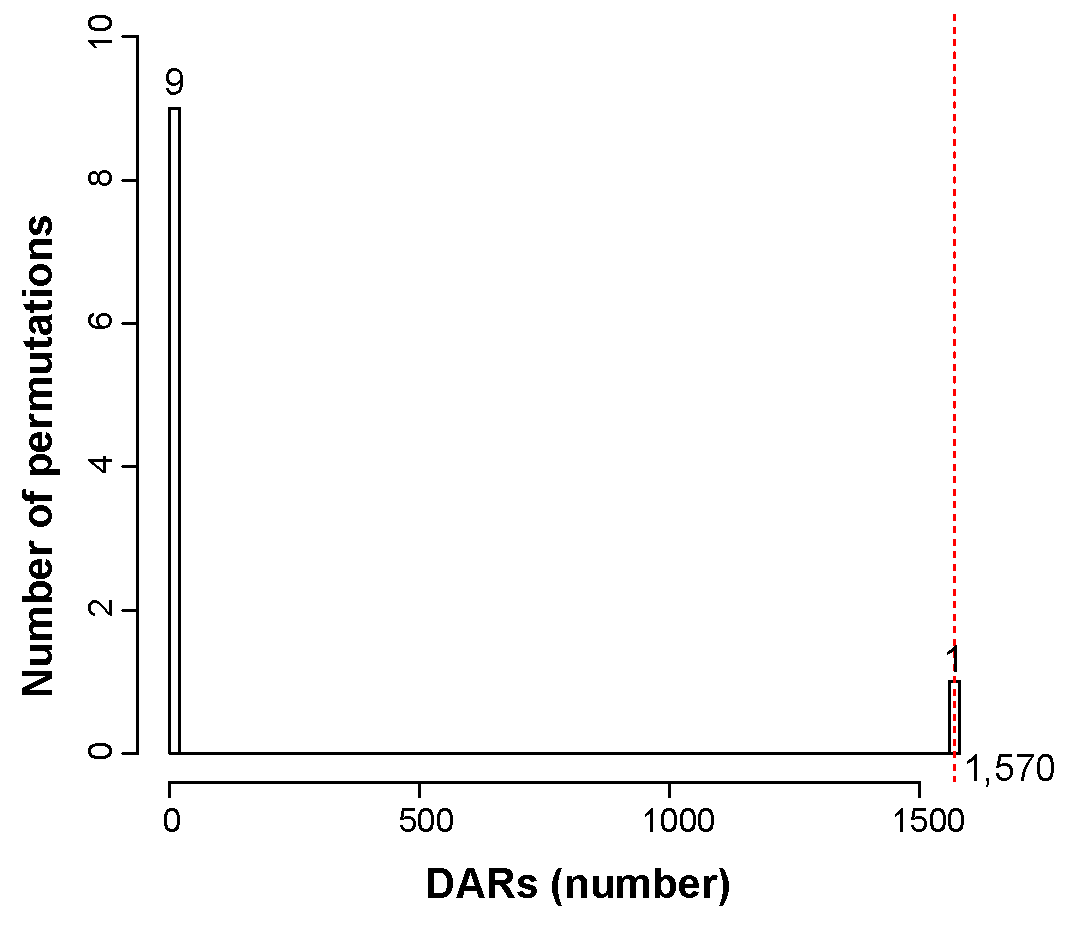
\includegraphics[width=\textwidth]{./Appendix/pdfs/Chapter5/ATAC_PsA_CD8_permutation_analysis}%
\caption{}
\end{subfigure}
\begin{subfigure}[b]{0.45\textwidth} 
%the [b] prevents offset in subcaptions
\centering
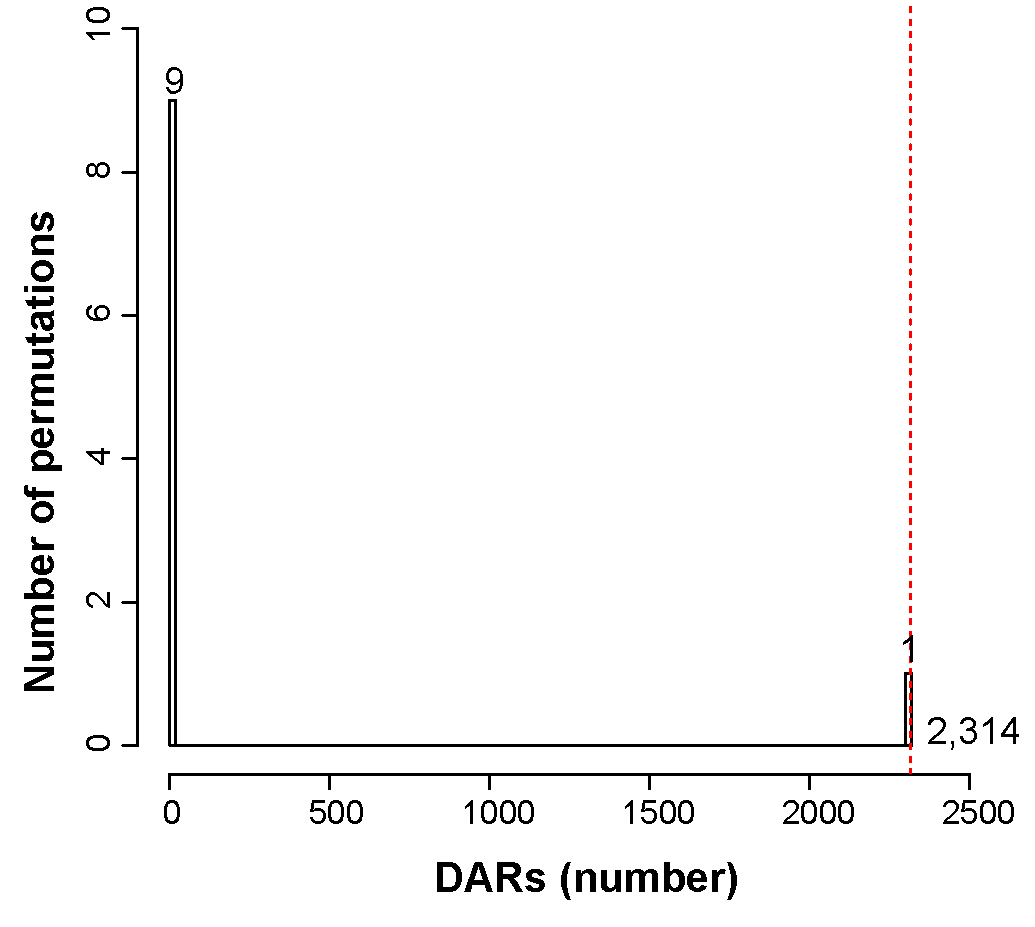
\includegraphics[width=\textwidth]{./Appendix/pdfs/Chapter5/ATAC_PsA_NK_permutation_analysis}%
\caption{}
\end{subfigure}
\caption[Permutation analysis SF vs PB in CD14$^+$,CD4m$^+$,CD8m$^+$ and NK.]{\textbf{Permutation analysis SF vs PB in CD14$^+$,CD4m$^+$,CD8m$^+$ and NK}. }
\label{figure:PsA_perm_analysis}
\end{figure}

\begin{figure}[htbp]
\centering
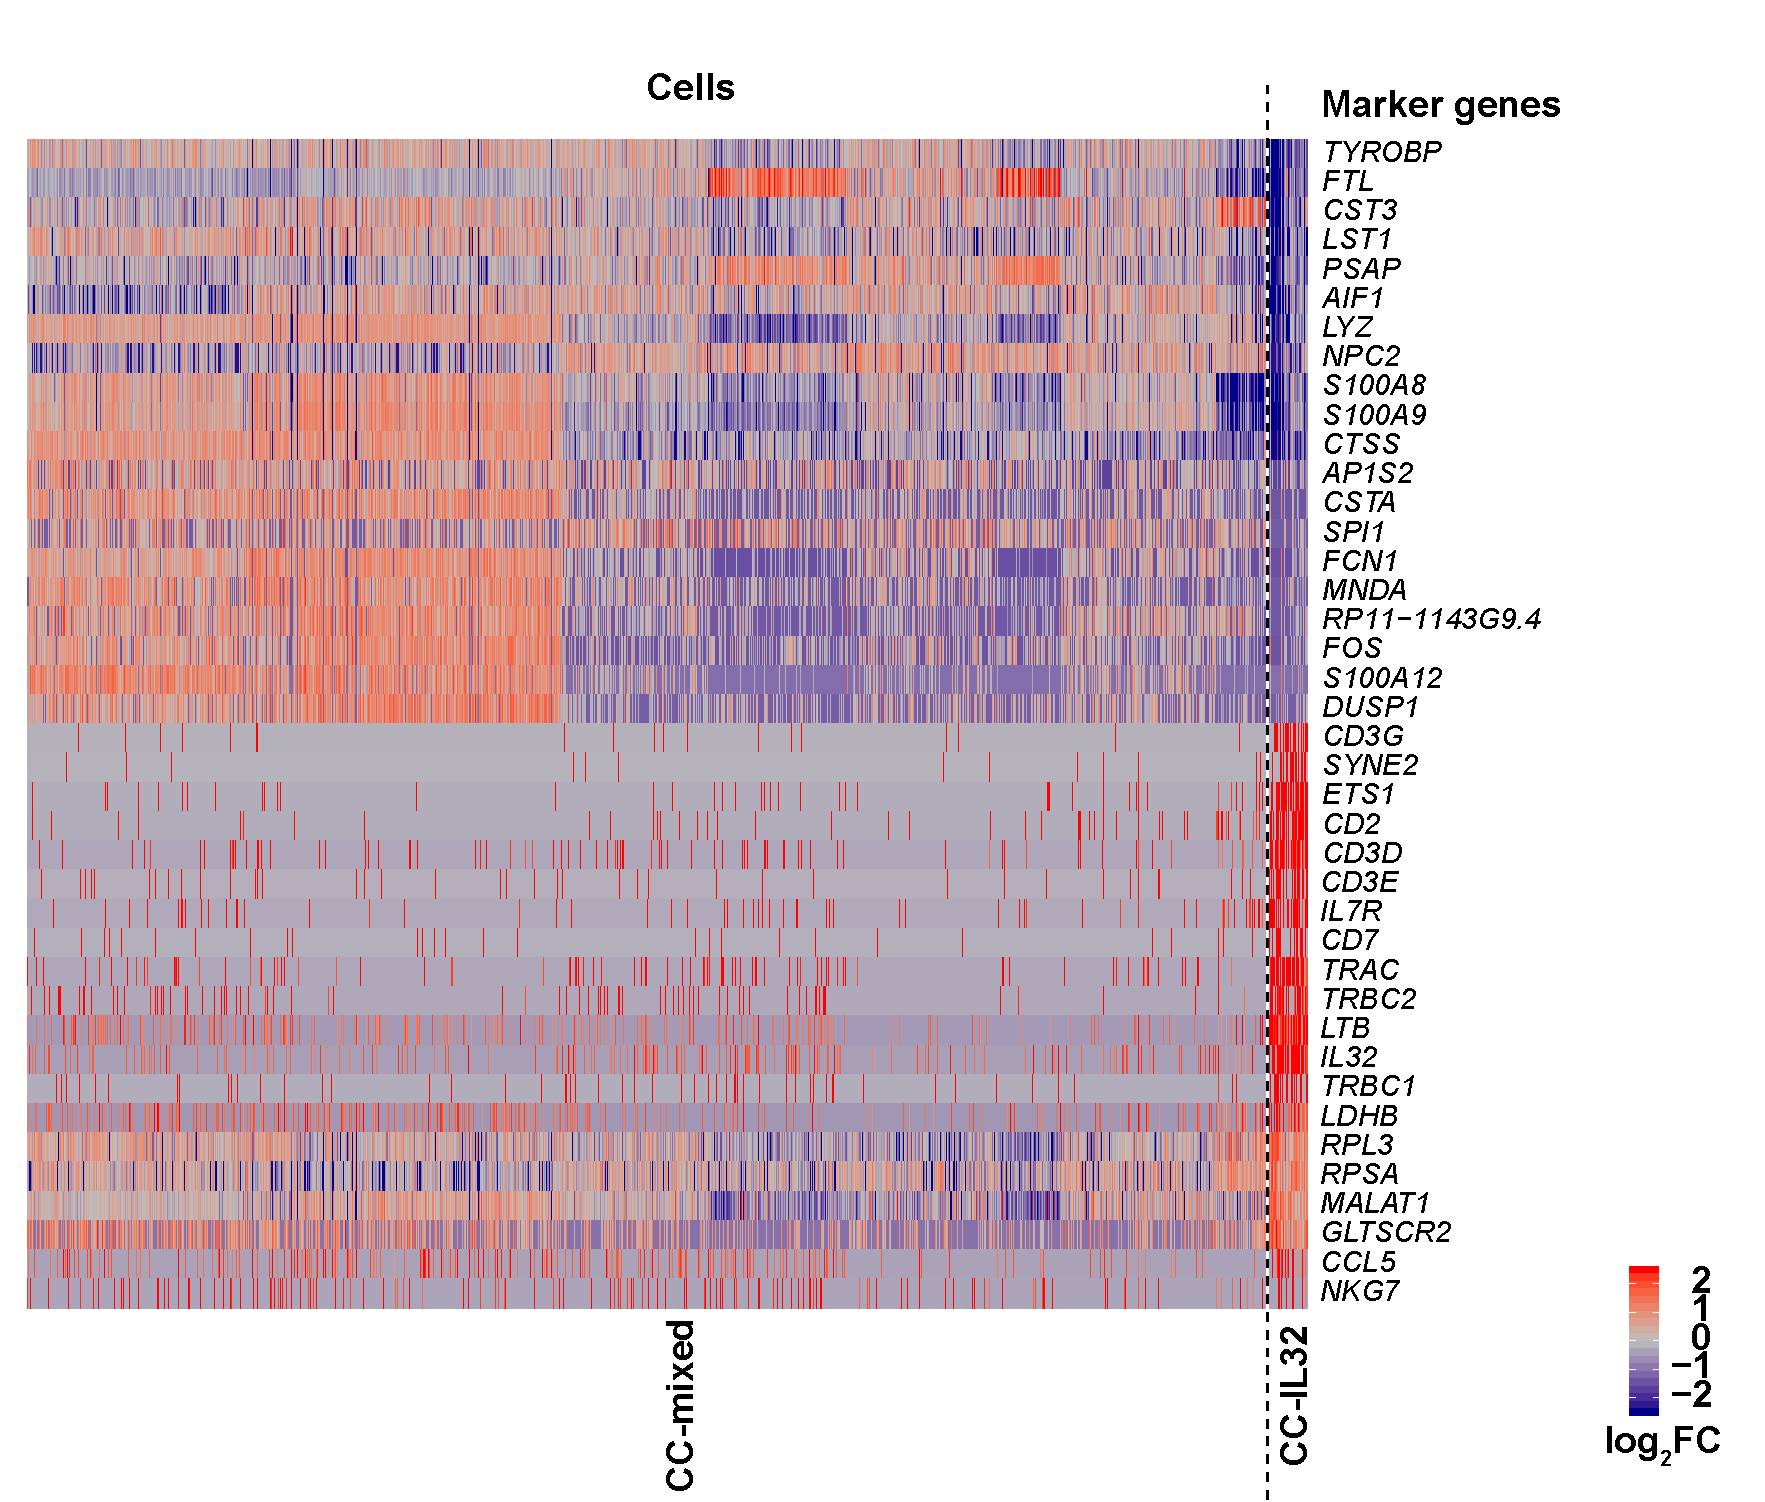
\includegraphics[width=0.6\textwidth]{./Appendix/pdfs/Chapter5/PSA_10X_heatmap_SF_PB_monocytes_clusters_mixed_and_IL7R}
\caption[Heatmap for the top 20 marker genes of the CC-mixed and CC-IL7R CD14$^+$ monocytes subpopulations.]{\textbf{Heatmap for the top 20 marker genes of the CC-mixed and CC-IL7R CD14$^+$ monocytes subpopulations.} Rows are the top 20 marker genes for each of the two subpopulations (total of 40 genes). The columns represent each of the cells members of the CC-mixed (left) or CC-IL7R (right) clusters. The colour scale represents the log$_2$FC in the expression of the marker gene in a particular cell of the cluster compared to the average expression of all the cells from the other cluster.}
\label{fig:PSA_scRNAseq_CC_mixed_and_IL7R_markers_heatmap}
\end{figure}

\bigskip
\begin{figure}[H]
\centering
\begin{subfigure}[b]{0.70\textwidth}
\centering 
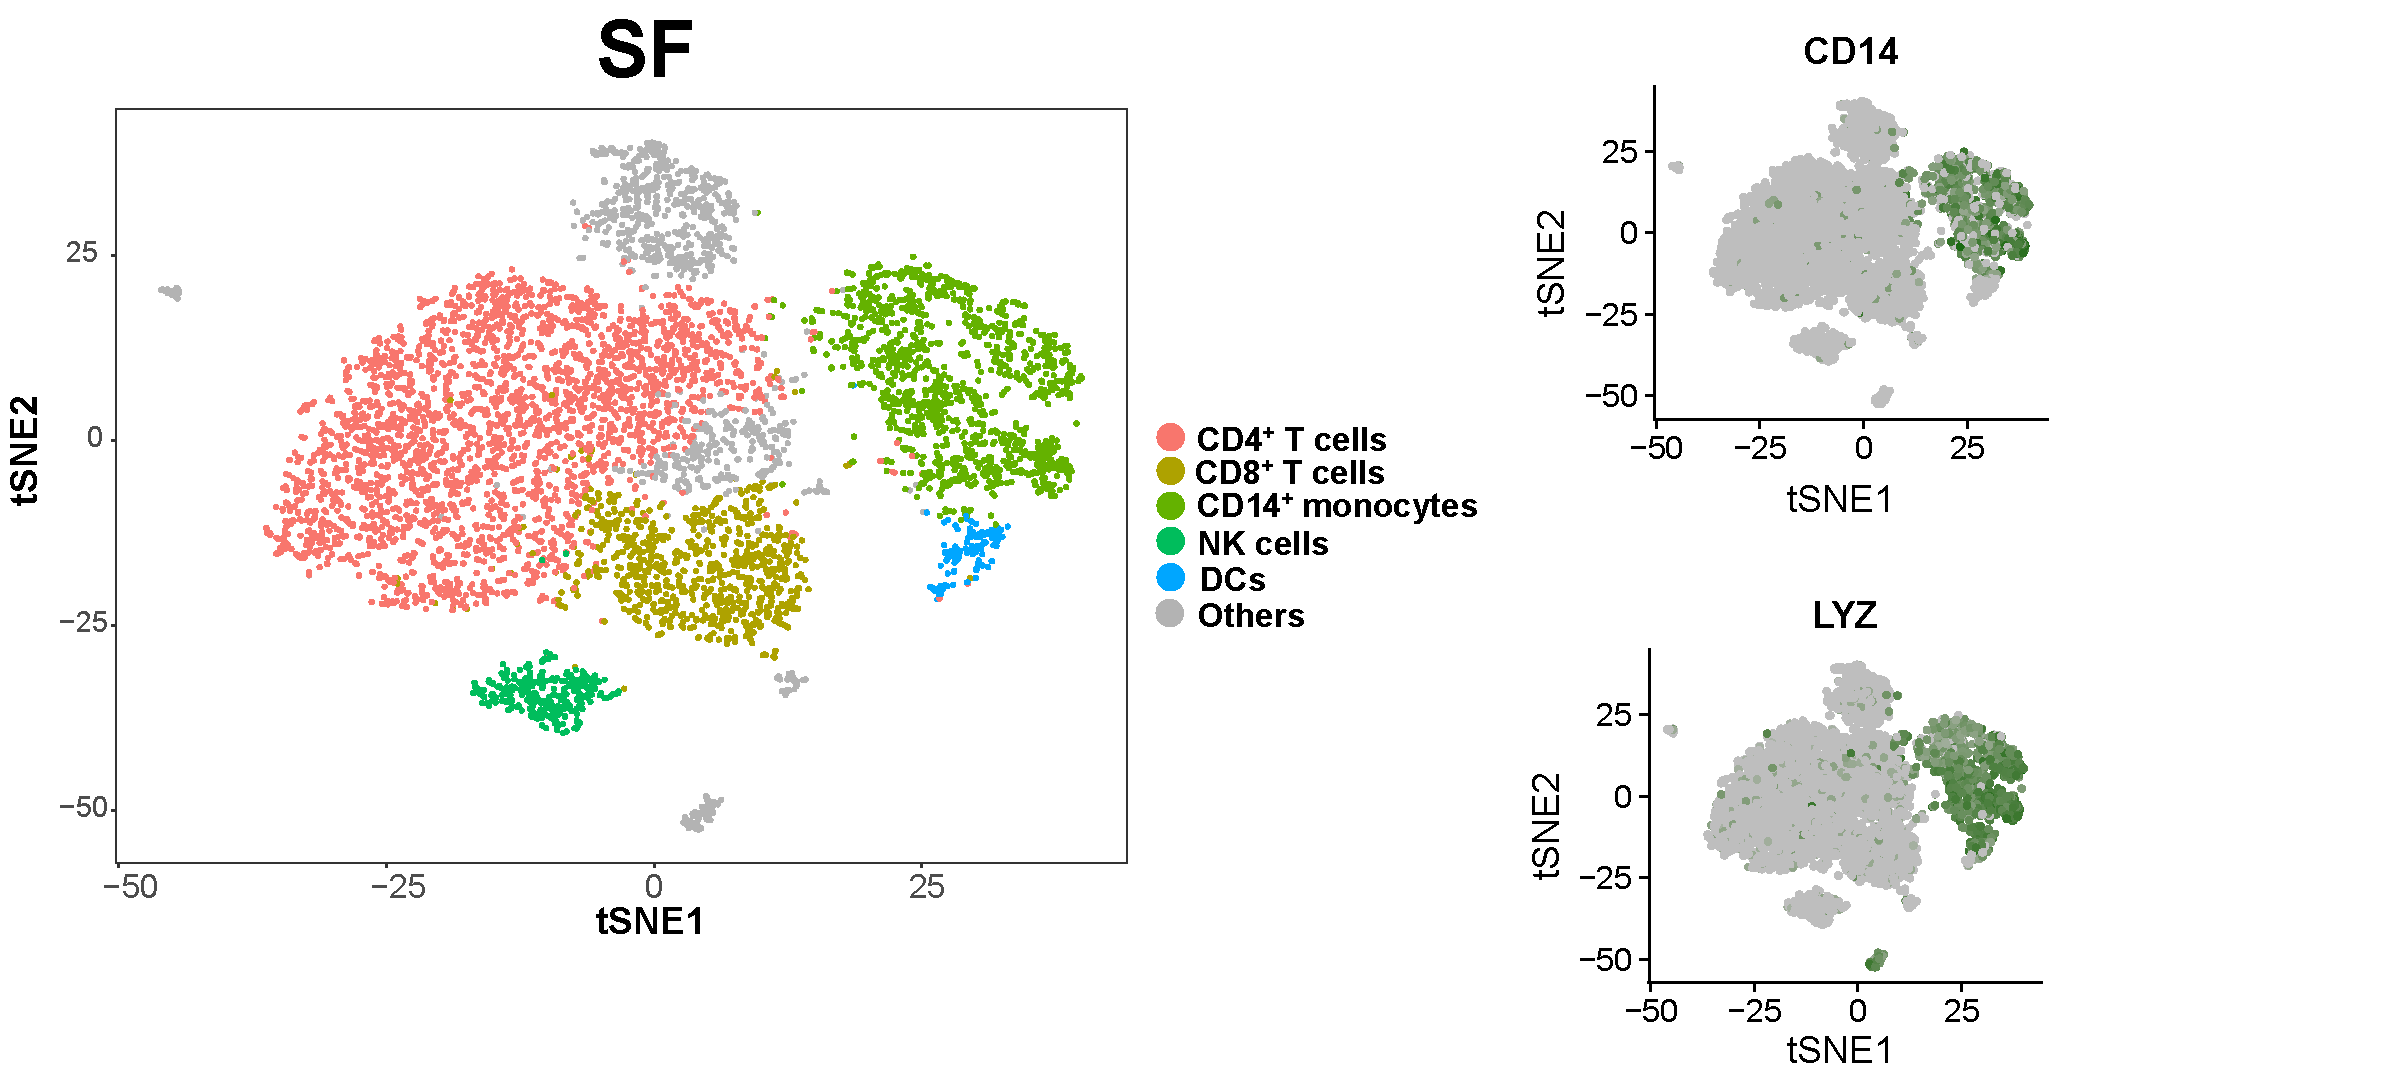
\includegraphics[width=\textwidth]{./Appendix/pdfs/Chapter5/PSA_SF_clusters_and_monocytes_markers}
\caption{}
\end{subfigure}
~
\begin{subfigure}[b]{0.70\textwidth} 
%the [b] prevents offset in subcaptions
\centering
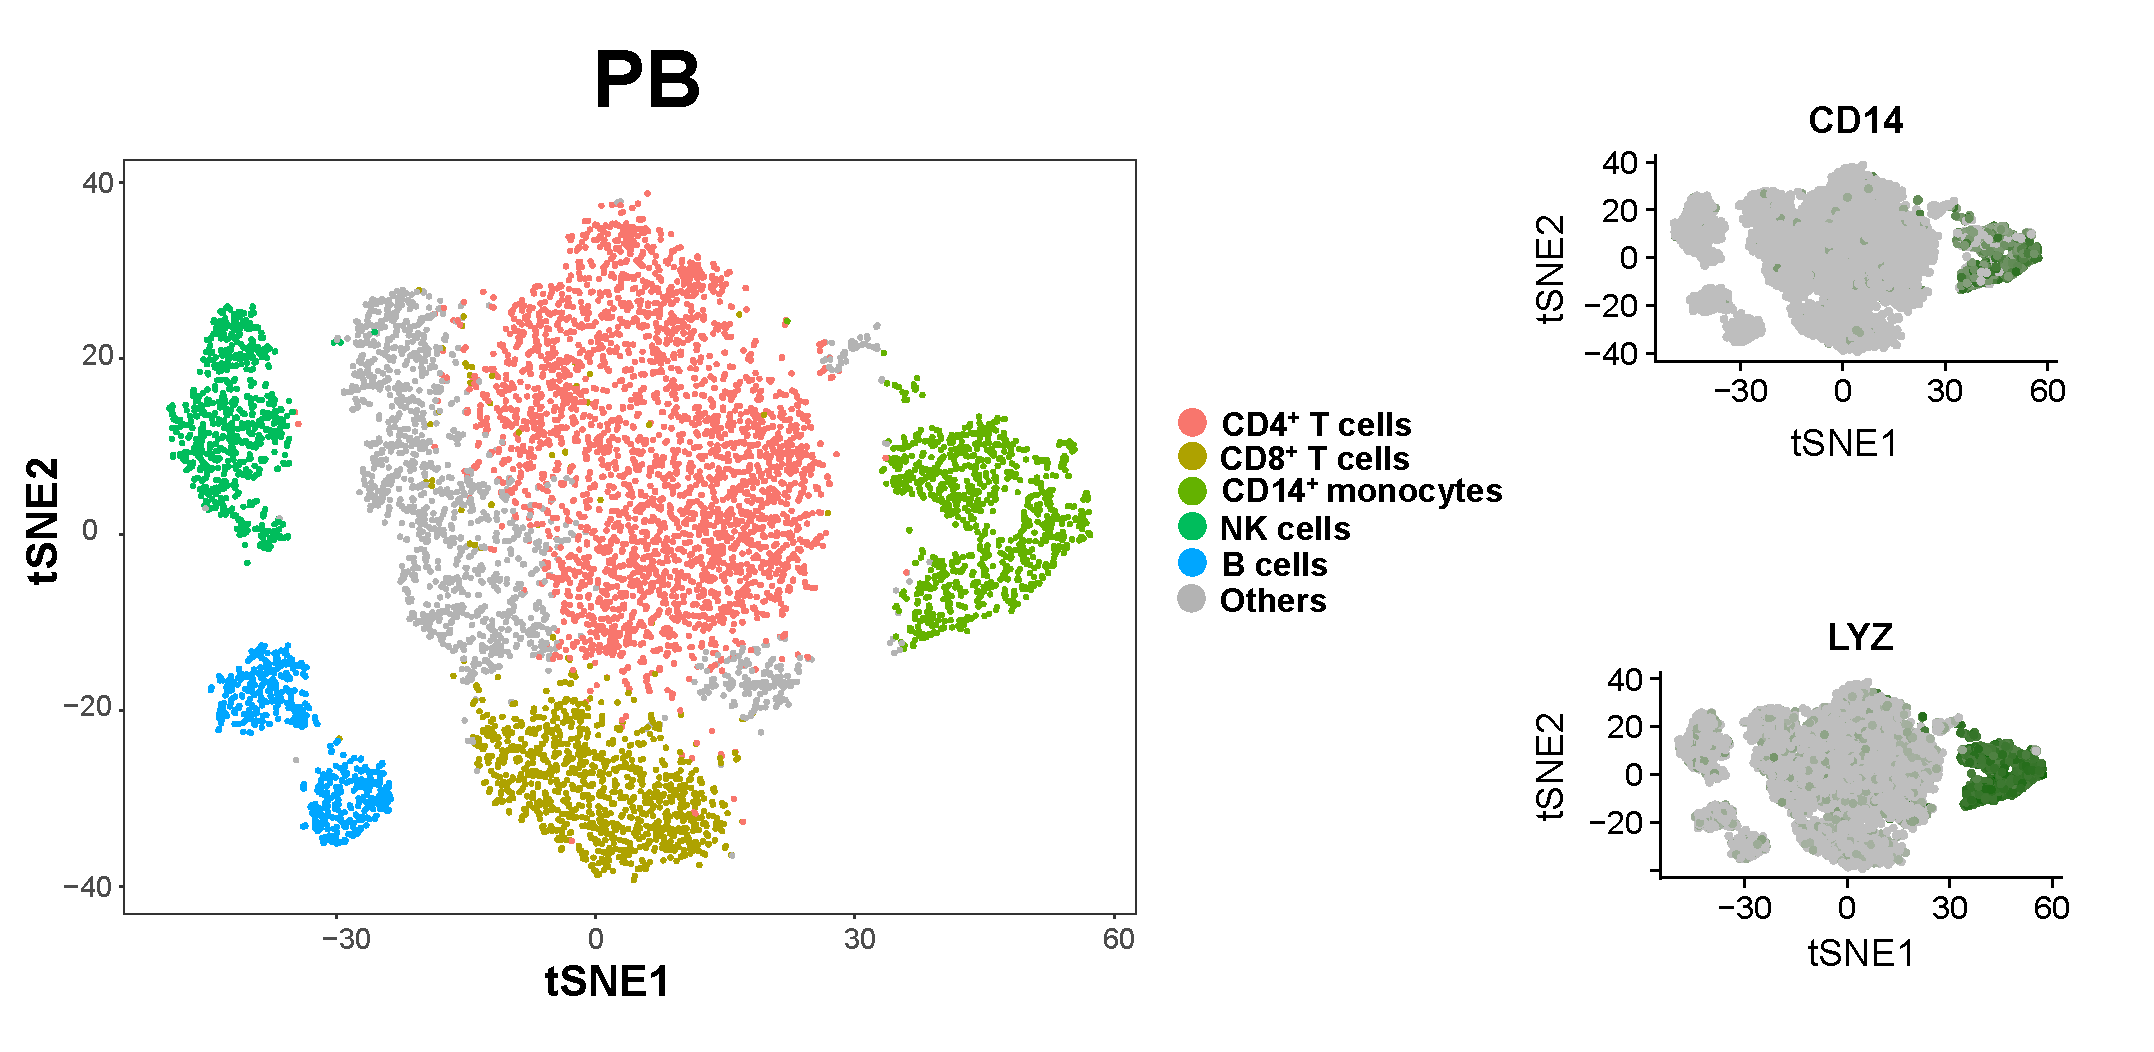
\includegraphics[width=\textwidth]{./Appendix/pdfs/Chapter5/PSA_PB_clusters_and_monocytes_markers}
\caption{}
\end{subfigure}
\caption[Identification of the CD14$^+$ monocytes populations from bulk SFMCs and PBMCs using scRNA-seq transcriptomes.]{\textbf{Identification of the CD14$^+$ monocytes populations from bulk SFMCs and PBMCs using scRNA-seq transcriptomes.} xxxx}
\label{figure:PsA_scRNAseq_SF_an_PB_monocytes_identification_from_bulk}
\end{figure}